% needs IEEEtran.cls
%
\documentclass[10pt,journal,compsoc]{IEEEtran}
%\documentclass[conference,compsoc]{IEEEtran}

\usepackage{graphicx}% Include figure files
%\usepackage{bm}% bold math
%\usepackage{gensymb}


%%%%%%%%%%%%%%%%%%%%%%%%%%%%%%%%%%%%%%%%%%%%%%%%%%%%%%%%%%%%%%%%%%%%%%%%%%%%%%%%
%%%%  Body of document follows...
%%%%%%%%%%%%%%%%%%%%%%%%%%%%%%%%%%%%%%%%%%%%%%%%%%%%%%%%%%%%%%%%%%%%%%%%%%%%%%%%
\begin{document}

\title{Quantum Domain Signals in Living Beings}

\author{Brad Eckert}
%\email{hwfwguy@gmail.com}
%\affiliation{Iolera Holdings LLC}

\date{\today}% It is always \today, today,
             %  but any date may be explicitly specified


\IEEEtitleabstractindextext{%
\begin{abstract}
We treat consciousness as a physical process occuring inside and outside of time
simultaneously, per spiritual traditions and recent scientific advances.
This view allows for two different dimensions of time.
Quantum time emerges from consciousness as it interacts with both worlds.
The relationship between the time dimensions provides a mechanism for flicker
noise arising from both our biological signaling and connection to divinity.
We present an algorithm for the demodulation of flicker noise.
Flicker noise can have discernible information content that instruments the
mind-body landscape.
The demodulated signals facilitate a new class of consciousness applications.
The detection and analysis of these signals has far-reaching implications for 
determinism, free will, heritability, and human interconnectedness.
\end{abstract}


% Note that keywords are not normally used for peerreview papers.
\begin{IEEEkeywords}
Tao, flicker noise, emergent time, consciousness.
\end{IEEEkeywords}}

\maketitle

%\tableofcontents

\input{../source/etime_intro}
\input{../source/etime_demod}
\section{Modulation}

Modulation is the reverse of demodulation.
It inputs a stream of (magnitude, angle) vectors and outputs a stream of real
samples. The downsample and upsample processes of modulation are the reverse
of demodulaton's upsample and downsample processes respectively.

\begin{figure}
	\centering
	\includegraphics[width=0.95\linewidth]{../source/mod_e}
	\caption[Causal to Emergent Time Demodulation]{Modulation data flow}
	\label{fig:mod}
\end{figure}

%%%%%%%%%%%%%%%%%%%%%%%%%%%%%%%%%%%%%%%%%%%%%%%%%%%%%%%%%%%%%%%%%%%%%%%%%%%%%%%%
\subsection{Downsampling}

V is downsampled to form frequency-domain signal U.
Eq. \ref{eq:eps_j} relates integer index $j$ to fractional index $\epsilon(j)$.
Each point of V can be interpolated into a variable number of U points in a way
that accumulates V points and spits out U points as needed.

Another view is easier to describe mathematically, but needs a logarithm. Let
$\epsilon$ and j be the respective indices of U and V where $\epsilon/j < 1$.
$\epsilon$ is an integer that steps downward from $\epsilon_0$.
\begin{equation}
\epsilon_0 = \frac{N}{2} - 1
\end{equation}

Rewriting equation \ref{eq:eps_j} for $j(\epsilon)$,

\begin{equation}  \label{eq:j_eps}
j(\epsilon) = \left(\frac{N}{2}-1\right)
ln\left(\frac{\epsilon_0}{\epsilon}\right)
\end{equation}

The minimum $\epsilon$ is determined by the span of j.
Let j range from 0 to $v-1$ and $v = 0.469N$.

\begin{equation}
\epsilon(v-1) = \epsilon_0 e^\frac{-(v-1)}{0.5N - 1}
\end{equation}

\begin{equation}
\epsilon(0.469N) = \epsilon_0 e^\frac{-(0.469N-1)}{0.5N - 1}
\approx 0.391 \epsilon_0
\end{equation}

Since $\epsilon$ is always positive, the upchirp case of $R>0$ needs to have its
j index mirrored by using V[v-j], where v is the maximum j such as 0.469N.

%%%%%%%%%%%%%%%%%%%%%%%%%%%%%%%%%%%%%%%%%%%%%%%%%%%%%%%%%%%%%%%%%%%%%%%%%%%%%%%
\subsection{IFFT}

The IFFT ($U \rightarrow Y$) is an Inverse Fast Fourier Transform that
translates N/2 complex frequency values to N/2 complex points in the causal
time domain. These may be assumed to have Hermitian symmetry,
so the imaginary part of $Y$ can be ignored.
It's also possible to realize Y as N real points.

A Hann window is applied to Y after the FFT. Y is then warped and accumulated
in X in a manner similar to the demodulator's correlation function.

%%%%%%%%%%%%%%%%%%%%%%%%%%%%%%%%%%%%%%%%%%%%%%%%%%%%%%%%%%%%%%%%%%%%%%%%%%%%%%%%
\subsection{Upsampling}

The upsampling process of Fig.~\ref{fig:mod} translates the sample pitch of
Y to the sample pitch of X using the reverse of the downsampling process.

Fig.~\ref{fig:upsam} illustrates an interpolation scheme for recreating X from Y.
The slope calculation requires a $1/\lambda$ scale factor.
The expense of division can be avoided by using another instance of exponential
sweep such as that described by Eq. \ref{eq:lambdaApprox}.

The X points are the trapezoidal area under the curve in Fig.~\ref{fig:upsam}.
The \textit{Head} and \textit{Middle} regions produce output points.
The \textit{Tail} result is carried into the next \textit{Head}.

\begin{figure}
	\centering
	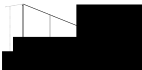
\includegraphics[width=0.8\linewidth]{../source/upsam_e}
	\caption[X interpolation]{Interpolation of Y for upsampling}
	\label{fig:upsam}
\end{figure}

Summation in X is similar to the data flow of Fig.~\ref{fig:wbuf},
but a little easier since X and Y are real (rather than complex) numbers.
X memory is wider than with demodulation to handle accumulation in memory.

\section{Implementation}

The algorithms are implemented in RTL (VHDL) for use on an FPGA or ASIC.
They may also be implemented in C, but certain functions are unwieldy on
typical computer hardware. For example, polar-to-rectangular and
rectangular-to-polar conversion is needed for upsampling complex numbers.
A simple test using GCC on a Core i7 took 1.6 $\mu$s per addition.
Table lookup (or other fast approximation) could speed that up:
Suppose 2x, so 800 ns.
In comparison, an RTL implementation using pipelined CORDIC can perform
one addition every two clocks. At 120 MHz, that's 17 ns.

A GPU could possibly process multiple data streams in parallel. 
However, FPGA is the cost/performance winner. 
The RTL algorithms lend themselves to multiple on-chip instances with very
little I/O. There's also a migration path to ASIC for when
``the new media'' takes off.

The RTL uses a CORDIC-based FFT with a throughput of about 7 clocks per sample.
Since the FFT dominates the processing time, downsampling and upsampling
are performed when the FFT is idle. This allows single-port RAM access and
sharing of the CORDIC hardware.
Overall throughput for a demodulator is about 12 clocks per input sample,
so about 10 MSPS. The input sample rate (such as from an ADC) is that divided
by the oversampling factor. For example, 100x oversampling results in
an ADC sample rate of 100 kSPS.

\begin{figure}
	\centering
	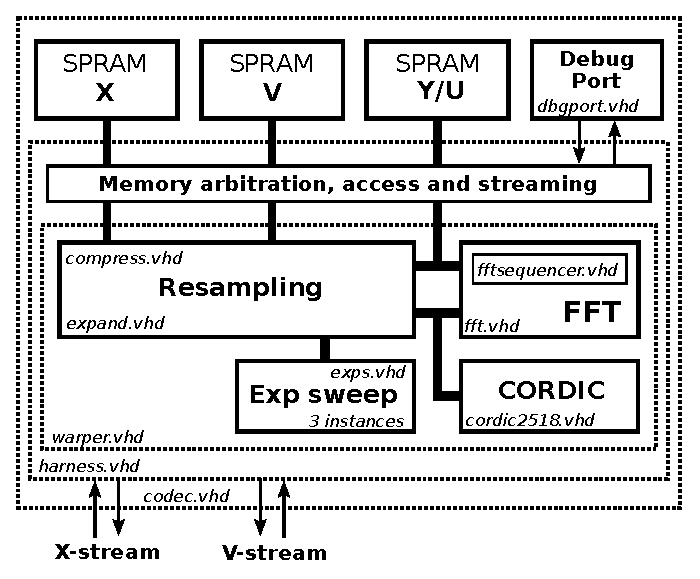
\includegraphics[width=0.8\linewidth]{../source/rtl_e}
	\caption[Emergent to Causal Time Hardware]{RTL Block Diagram}
	\label{fig:rtl}
\end{figure}

\subsection{Instrumentation}

The test port uses a half-duplex byte-oriented streaming protocol to access
hardware features for testing, verification, and debugging.
If necessary, the I/O streams may also be handled through the test port.
It uses all byte codes between 00 and FF, except for 10 to 13,
which are reserved for embedded ``escape sequences'' and flow control.
This strategy allows for XON/XOFF flow control if a UART is used as the PHY.
The PHY may be a USB FIFO chip (such as FT232H), SPI, UART, JTAG, or TWI.

The test port is used with test apps to verify separate steps of the
algorithm such as downsample, FFT, upsample, etc.
Connection to a test PC through a 2-wire UART is sufficient for FPGA testing.
The entire transform is coded in vanilla VHDL for ease of porting.

The demodulator/modulator shown in Fig.~\ref{fig:rtl} uses three memory
spaces to allow easier I/O access by the I/O streams and account for the
difference in word widths between X and V data.
The \verb|warper| uses wide data busses on the X and V memories to facilitate
correlation of outgoing data using long accumulators in either X or V memory.
Incoming data is packed two points per memory word.

\subsection {FPGA utilization}

A complete CODEC was implemented in vanilla VHDL with a single clock domain.
Free versions of synthesis tools were used to synthesize the design for use in
some sample FPGAs. 
The clock rate is limited by the exponential sweep module, 
which uses a single-cycle feedback loop whose path includes a 26x27 multiplier,
4:1 mux, adder, and 3:1 mux. Those two muxes will do better on FPGAs with 
6-input LUTs. Synthesis for parts with LUT6 had a 50\% reduction in LUT usage
compared to LUT4-only.

\begin{table}[t]\centering
	\label{tab:FPGAfit}
	\caption{FPGA rough synthesis results. One-off distributor pricing gives a 
	rough cost per MHz, using Digikey pricing, across the number of CODEC 
	instances that will fit in the FPGA.}
	\centering
	\begin{tabular}{lccrrr}
		\hline\hline
		Device & Logic & DSPs & Clock & Cores & \$/MHz\\ [0.5ex]
		\hline
        Artix 7   & 8K LUT6 & 40   & 150 MHz & 12 & 0.11\\
		Cyclone 10& 14K LE & 69 9x9 & 49 MHz &  4 & 0.25\\
		LFE5      & 12K LE & 40     & 39 MHz &  1 & 0.30\\
        PolarFire & 14K LUT4 & 37   & 51 MHz &  7 & 0.40\\
		Cyclone 5 & 5K ALM & 18     & 72 MHz &  2 & 0.55\\
		MAX10     & 13K LE & 69 9x9 & 51 MHz &  1 & 1.20\\
		\hline
	\end{tabular}
\end{table}



\bibliographystyle{IEEEtran}
\bibliography{IEEEabrv,../source/etime}

\end{document}

